%\documentclass[../main.tex]{subfiles}
%\begin{document}
\emph{Process mining} is a relatively new discipline that bridges the gap of data mining and business process management. The objective of process mining is to support the analysis of business processes, provide valuable insights in processes and further improve the business execution based on the business execution data which is recorded in event logs. According to  \cite{van2011process}, process mining techniques are divided into three categories: \emph{process discovery}, \emph{conformance checking}, and \emph{process enhancement}. \emph{Process discovery} techniques derive visual models from event logs of the information system, aiming at a better understanding of real business processes. \emph{Conformance checking} analyzes the deviations between a referenced process model and observed behaviors driven from its execution. \emph{Process enhancement} adapts and improves existing process models by extending the models with additional data perspectives or repairing the reference models to accurately reflect observed behaviors. 

Most of the organizations have predefined process execution rules which are captured in a process model. However, in real life, business processes often encounter exceptional situations where it is necessary to execute process differing from the reference model. To reflect reality, the organizations need to adjust the existing process model. Basically, one can apply process discovery techniques again  on the event log to obtain a new model only based. This method is referred as process rediscovery. However, there is a need that the improved model should be as similar as possible to the original model while replaying the current process execution \cite{fahland2012repairing}. In this situation, the rediscovery method tends to fail due to the ignorance of the impact from the existing model. To meet this need, \textbf{model repair} techniques are proposed in  \cite{fahland2012repairing}.

\emph{Model repair} belongs to process enhancement \cite{fahland2012repairing}. It analyzes the workflow deviations between an event log and a process model, and fixes the deviations mainly by adding subprocesses on the model. As known, organizations are goal-oriented and aim to have high performance according to a set of Key Performance Indicator(KPI)s, e.g. the production time for a car industry, the logistic cost for importer companies.  However, little research in process mining is conducted on the basis of business performance \cite{ghasemi2019event}.  The authors of  \cite{ghasemi2019event} point out several contributions e.g.   \cite{dees2017enhancing} to consider business performance into process mining. The work in  \cite{dees2017enhancing} divides deviations of model and the event log into positive and negative according to certain KPIs. Then it applies repair techniques in  \cite{fahland2012repairing} only with positive deviations which are deviations leading to positive KPI outcomes. This reason behind this approach  is to avoid introducing negative instances into the repaired model. 

However, the current repair methods have some limits. Model repair techniques fix the model by adding subprocesses. They guarantee that the repaired model replays the whole event log but overgeneralizes the model, such that more behaviors are allowed than expected. Furthermore, the model complexity is increased by the repair techniques in \cite{fahland2012repairing}.  Even the performance is considered in  \cite{dees2017enhancing}, but only positive deviations are used to add subprocesses, the negative information is ignored, which disables the possibility to block negative behaviors from model. 

In the following sections, motivating examples are given to describe those limits of the current repair techniques in several situations. Then we propose research questions to overcome those limits and define our research scope. At the end, we give the outline for the whole thesis.
%% Motivation 
\section{Motivating Examples}
\begin{wrapfigure}{r}{0.3\textwidth}
	\centering
	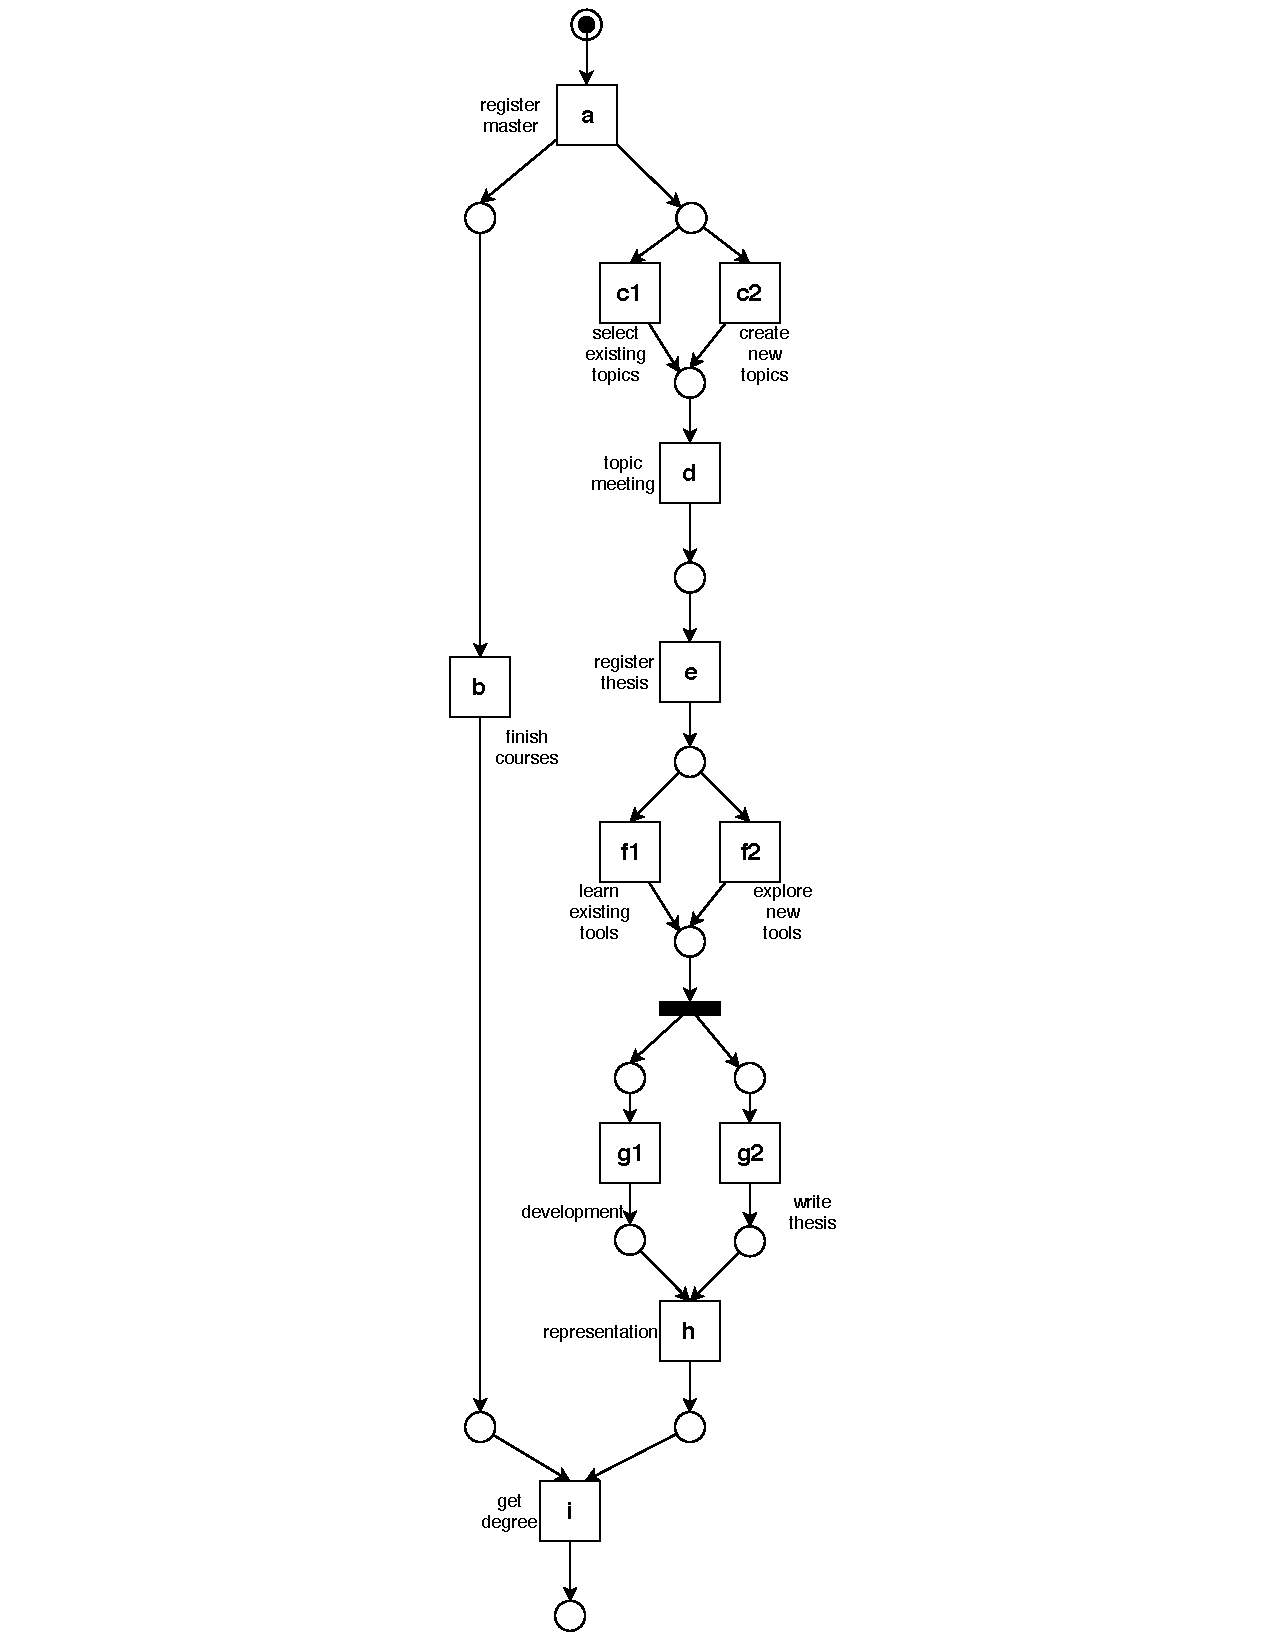
\includegraphics[clip, trim=7cm 0cm 7cm 0cm, width=0.4\textwidth, height=0.7\textheight]{figures/introduction/Master-original-model.pdf}
	\caption{original master study process $M_0$}
	\label{fig:model_M0}
\end{wrapfigure}
% In this section, we use thesis registration example to display the shortcomings of existing techniques and then introduces our methods, but we need to answer them later..
This section describes some situations where current repair techniques tend to fail. To benefit better understanding, examples are extracted from the common master study procedure to illustrate those situations.

The main activities for the master study include \textbf{register master}, \textbf{finish courses} and \textbf{write a master thesis}. Here, we simplify the \textbf{finish courses} and only extend the activity \textbf{write a master thesis} into a set of sub activities. Those activities are shown in the Petri net model $M_0$ of Figure \ref{fig:model_M0}. The activities are modeled by the corresponding \textbf{\textbf{transitions}} which are represented by squares. Transitions are connected through \textbf{\textbf{place}} represented in circles. Transitions and places build the static structure of Petri net and describe the transition relations. \textbf{\textbf{Tokens}} in the black dot are put in places and represent the dynamic state of the model. 

$M_0$ is currently in an initial state where one token is at the start place to enable the transition \textbf{register master}. After firing \textbf{register master}, the token at the initial place is consumed while two new token are generated in the output places of \textbf{register master}. In this way, activity \textbf{finish courses}  can be executed concurrently with the parallel branches. When multiple activities have the same input place, all of them are enabled but only one of them can be fired and executed, namely, they are exclusive to each other. As shown in the figure,  \textbf{select existing topics}  and \textbf{create new topics} are exclusive, and only one of them can be triggered. When a transition has multiple input places, it can be triggered with condition that all input places hold at least a token. \textbf{Get degree} is enabled only after \textbf{finish courses} and \textbf{presentation} are completed. 


% here we are going to talk about the situations where the current repair method can not handle well.
%talk about the execution trace definition. 
% but how to combine them into one example?? I don't think it clearly here. But I need to show it later.
As the tokens flow through the model, activities get fired and generate a sequence according to their execution order. One execution sequence is called a trace. A set of traces depicts the model behavior and is recorded into a data file called event log. In real life, activities might be executed with deviation to the process model. A trace which has no deviation to the model is a fitting trace. Otherwise, it's an unfitting trace. With accumulation of deviations, process model needs amending to reflect reality.  In the following part, In the following part,
several situations are introduced to demonstrate the shortcomings of current techniques
to repair a model.
\iffalse
\begin{align*}
L= \{ & { <a,b, c1,d,\textbf{x1}, e,f1,g1,g2,h,i>}^{50, pos}, \\   
      &{<a,b, c2,d,\textbf{x2},e,f2,g2,g1,h,i>}^{50, pos}, \\
      &{<a,b, c1,d,\textbf{x2},e,f1,g2,g1,h,i>}^{30, pos}, \\
      &{<a,b, c1,d,\textbf{x2},e,f1,g2,g1,h,i>}^{20, pos}, \\
      
      &{<a,\quad c1,\quad d,e,f1,g2,g1,h,i>}^{50, neg}, \\
      &{<a,\quad c1,b, d,\textbf{x2},e,f1,g2,g1,h,i>}^{50, neg}, \\
      &{<a,\quad c1,d,b, e,f2,g2,g1,h,i>}^{50, neg}, \\
      
\}
\end{align*}
\fi
%% here we want to use one example to show the shortcomings of current repair methods.. How to organize them??? 
\subsection{Situation 1: \small{Repairing Model with Unfitting Traces}} % add preparation to this model
In some universities, before registering a master thesis, the activities \textbf{write proposal} and \textbf{check course requirement} with exclusive choice relation might be necessary in the master study procedure. The real process are recorded in the event log $L_1$. Traces with either of those activities are considered as positive. For convenience, alphabet characters are used to represent the corresponding activities and annotated in the model. \textbf{x1, x2} represent the activities \textbf{write proposal} and \textbf{check course requirement}.
		\begin{align*}
		L_1:= \{ &  {<a,b,c1,d,\textbf{x1},e,f1,g1,g2,h,i>}^{50, pos}, \\   
		             &{<a,b,c2,d,\textbf{x2}, e, f2,g2,g1,h,i>}^{50,pos} \}
		% Negative: \{ & {<a,c1,d,\quad f,g1,g2,h,i>}^{50} \}
		\end{align*}
\begin{figure}[htp]
	\centering
	\begin{subfigure}[b]{0.48\textwidth}
		\centering
		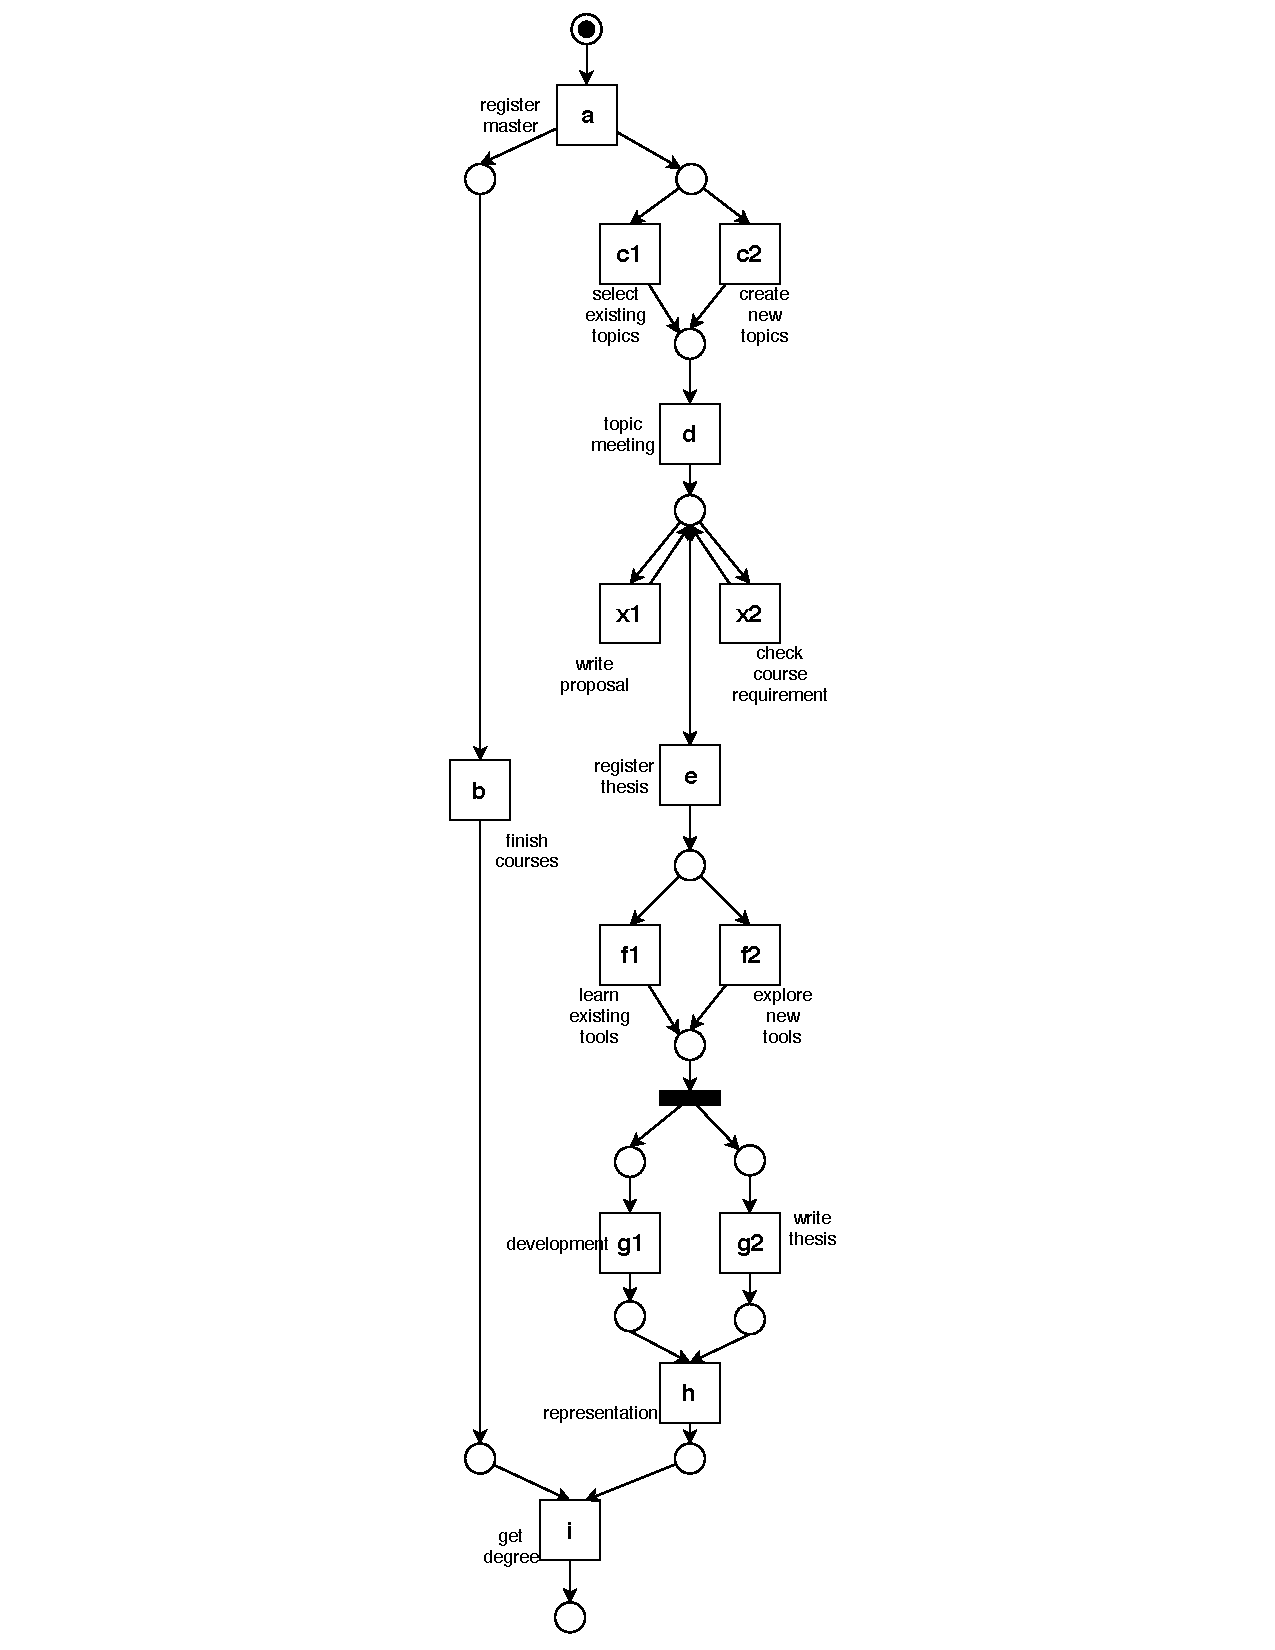
\includegraphics[clip, trim=7cm 0cm 7cm 0cm, width=0.5\linewidth, height=0.7\textheight]{figures/introduction/Master-add-events-loop.pdf}
		\caption{repaired model $M_{1.1}$ with techniques in \cite{fahland2015model}}
		\label{fig:model_b1}
	\end{subfigure}%
	\begin{subfigure}[b]{0.48\textwidth}
		\centering
		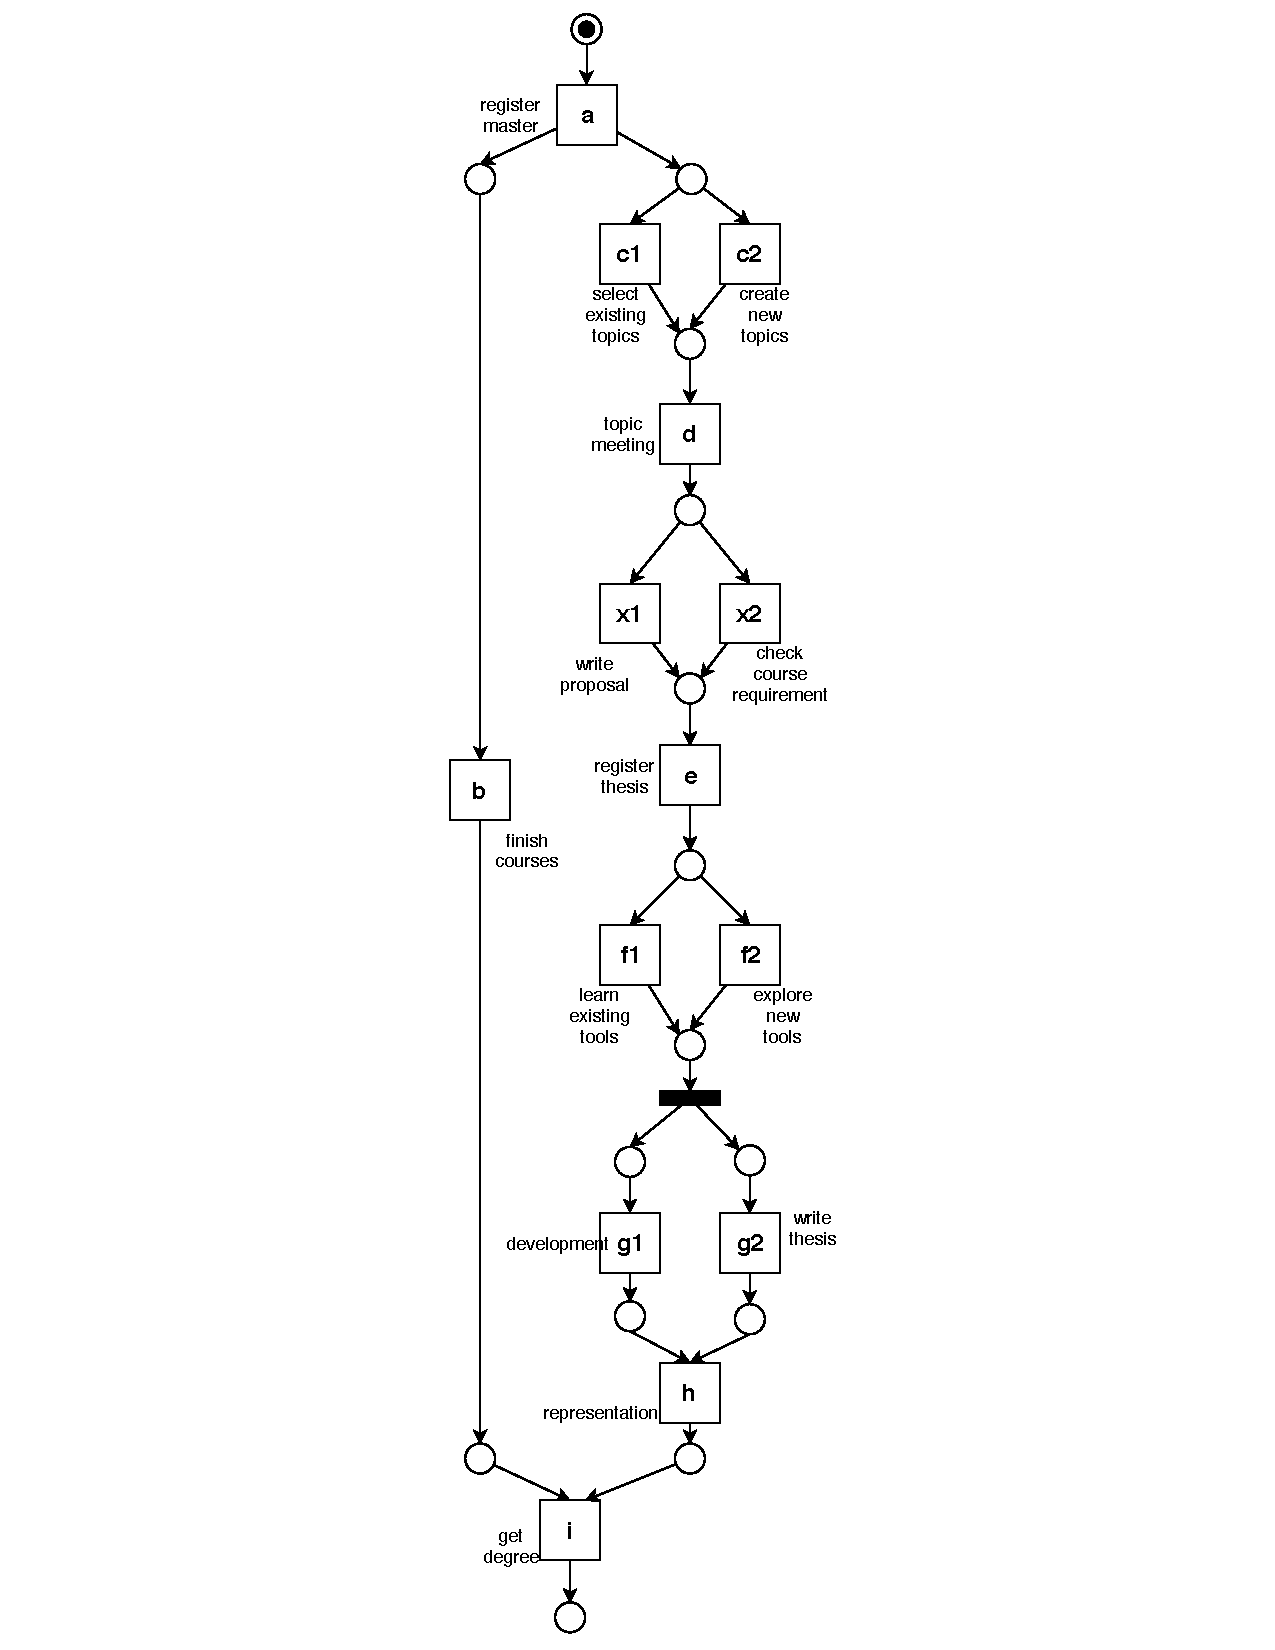
\includegraphics[clip, trim=7cm 0cm 7cm 0cm, width=0.5\linewidth, height=0.7\textheight]{figures/introduction/Master-add-events.pdf}
		\caption{expected model $M_{1.2}$}
		\label{fig:model_b2}
	\end{subfigure}
	\caption{example for situation 1 where $M_{1.1}$ is repaired by adding subprocess in the form of loops, which results in lower precision compared with the expected model $M_{1.2}$.}
	\label{fig:model_change_1}
\end{figure}
Because the existing repair techniques  \cite{fahland2015model} don't consider the performance of traces in event log, all instances with positive labels are used to repair the model. Firstly, the deviations of the existing model M0 and the event log $L_1$ are computed. After computation of deviations, each deviation has the same start and end place and two deviations appear at the same position in the model. When repairing this model, each subprocess has one place as its start and end place, which forms a loop in the model. If there is only one such subprocess, the subprocess is added in a sequence in the model, which leads to a higher precision. Yet the algorithm does not discover orders between different subprocesses at overlapping locations. So the subprocesses are kept in a loop form. 

The repaired model is shown in Figure \ref{fig:model_b1}, where the two additional activities are added in the form of loop. The repair algorithm in  \cite{dees2017enhancing} builds upon  \cite{fahland2015model} and considers the performance of the event log. However, the repaired model is the same as the one in Figure \ref{fig:model_b1}. The reasons are: (1) there is no deviation from negative factors. (2) positive deviations are used in the same way as  \cite{fahland2015model}. 

Compared to the model in Figure \ref{fig:model_b1} where the two extra activities are shown in loop, the model in Figure \ref{fig:model_b2} is more expected with \textbf{x1, x2} in sequence and a higher precision.

\subsection{Situation 2: \small{Repairing A Model with Fitting Traces}}
% we should delete the prepare carefully and casually from the model. Only consider to add the data about the order change..what we expect is not 
This situation describes the existing problem in the current methods that fitting traces with negative performance outcomes cannot be used to repair a model. Given an actual event log $L_2$, when activity \textbf{finish courses} is fired after \textbf{begin thesis} and before writing master thesis, it reduces the pressure for the master thesis phase. Traces in such case are treated as positive.
\begin{align*}
L_2:=\{ & { <a,\textbf{b},c1,d,e,f1,g2,g1,h,i>}^{50, pos} , \\   &{<a,\textbf{b},c2,d,e,f2,g1,g2,h>}^{50, pos};   \\
& {<a,c1,d,e,f2,g2,g1,\textbf{b},h,i>}^{50, neg} , \\
& {<a,c1,\textbf{b},d,e,f1,g1,g2,h,i>}^{50, neg}  \}
\end{align*}
Compared to $M_0$, the event log $L_2$ contains no deviation. When we apply the techniques in  \cite{fahland2015model} and  \cite{dees2017enhancing} to repair the model, the model remains unchanged. Apparently, the fact that those two methods can't incorporate the negative information in fitting traces causes this shortcoming. A model as $M_2$ is expected because it enforces the positive instances and avoids the negative instance. Unfortunately, the current methods don't allow us to obtain such results. 
\begin{figure}[htp]
	\centering
	\begin{subfigure}[b]{0.5\textwidth}
		\centering
		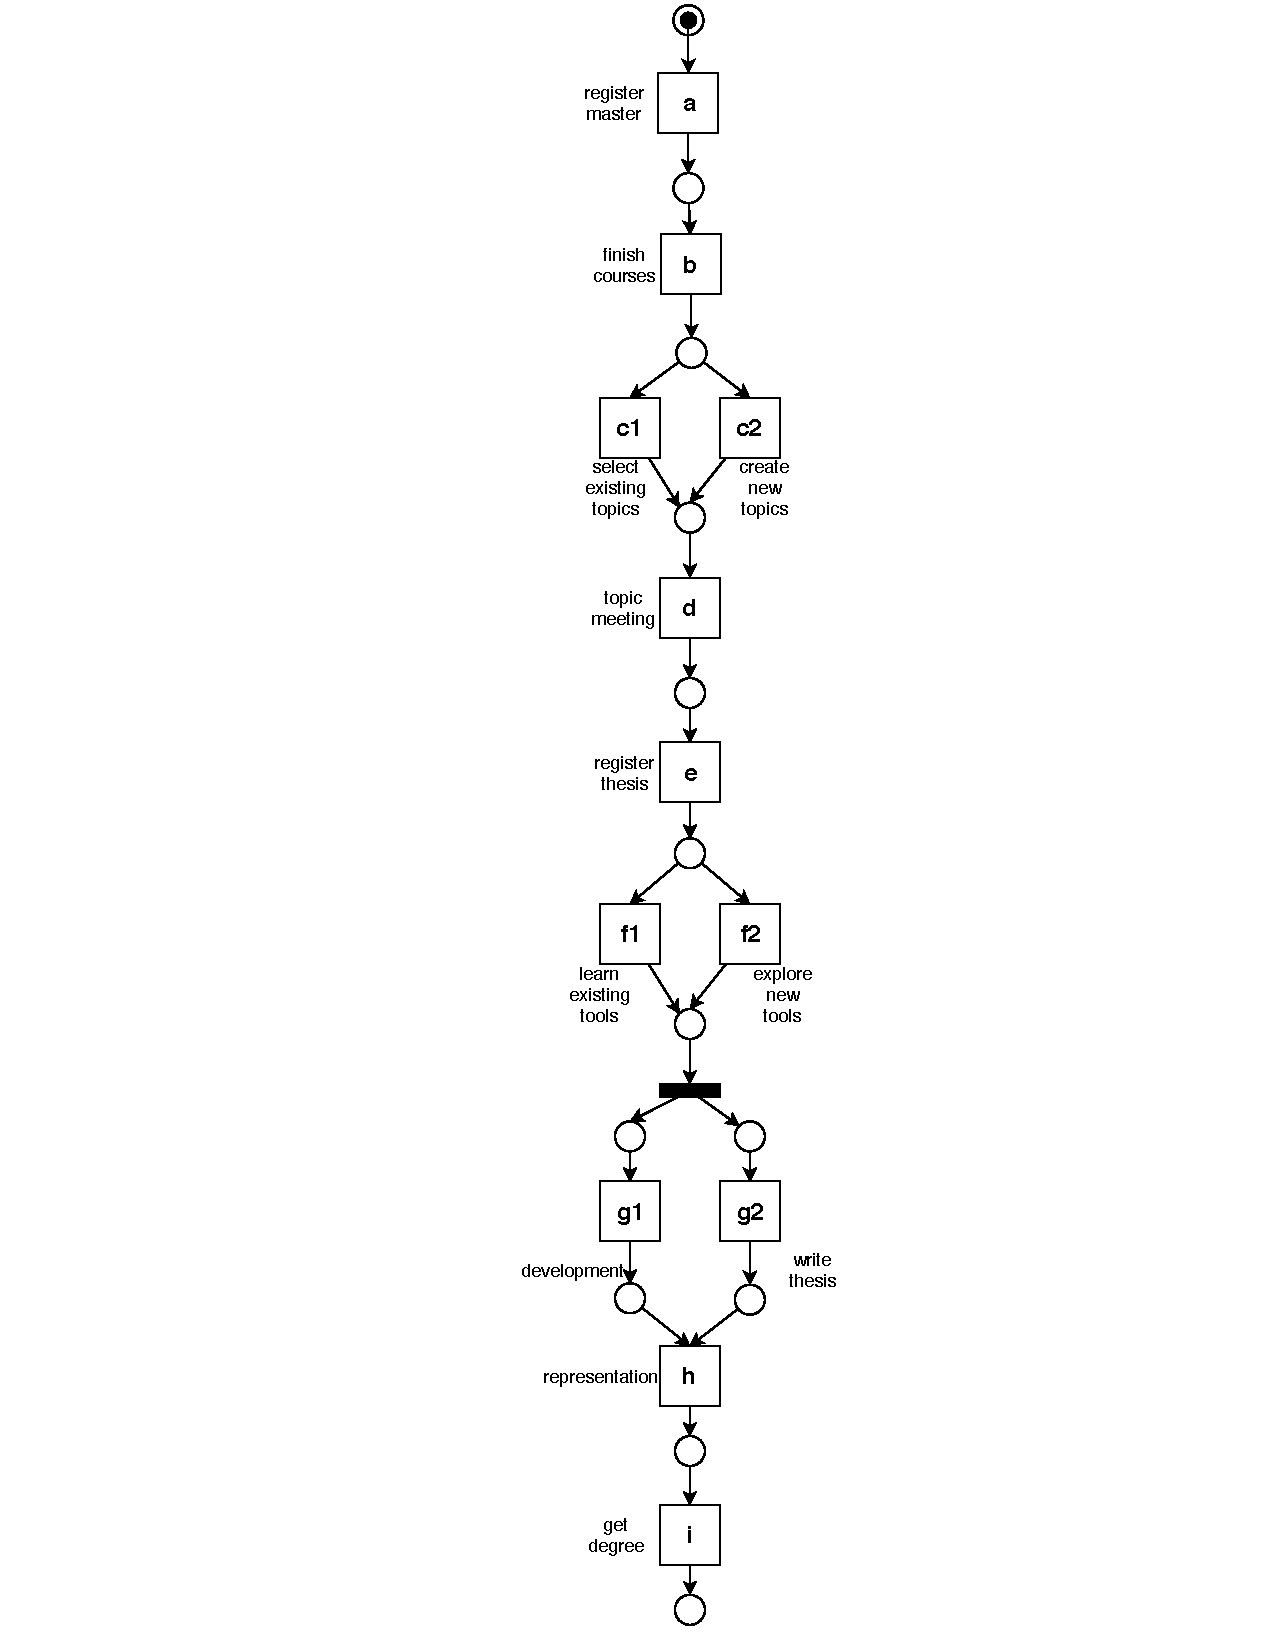
\includegraphics[clip, trim=8cm 0cm 8cm 0cm, width=0.5\linewidth, height=0.7\textheight]{figures/introduction/Master-change-order.pdf}
		\caption{expected model $M_{2}$ with order change}
		\label{fig:model_c}
	\end{subfigure}%
	\begin{subfigure}[b]{0.5\textwidth}
		\centering
		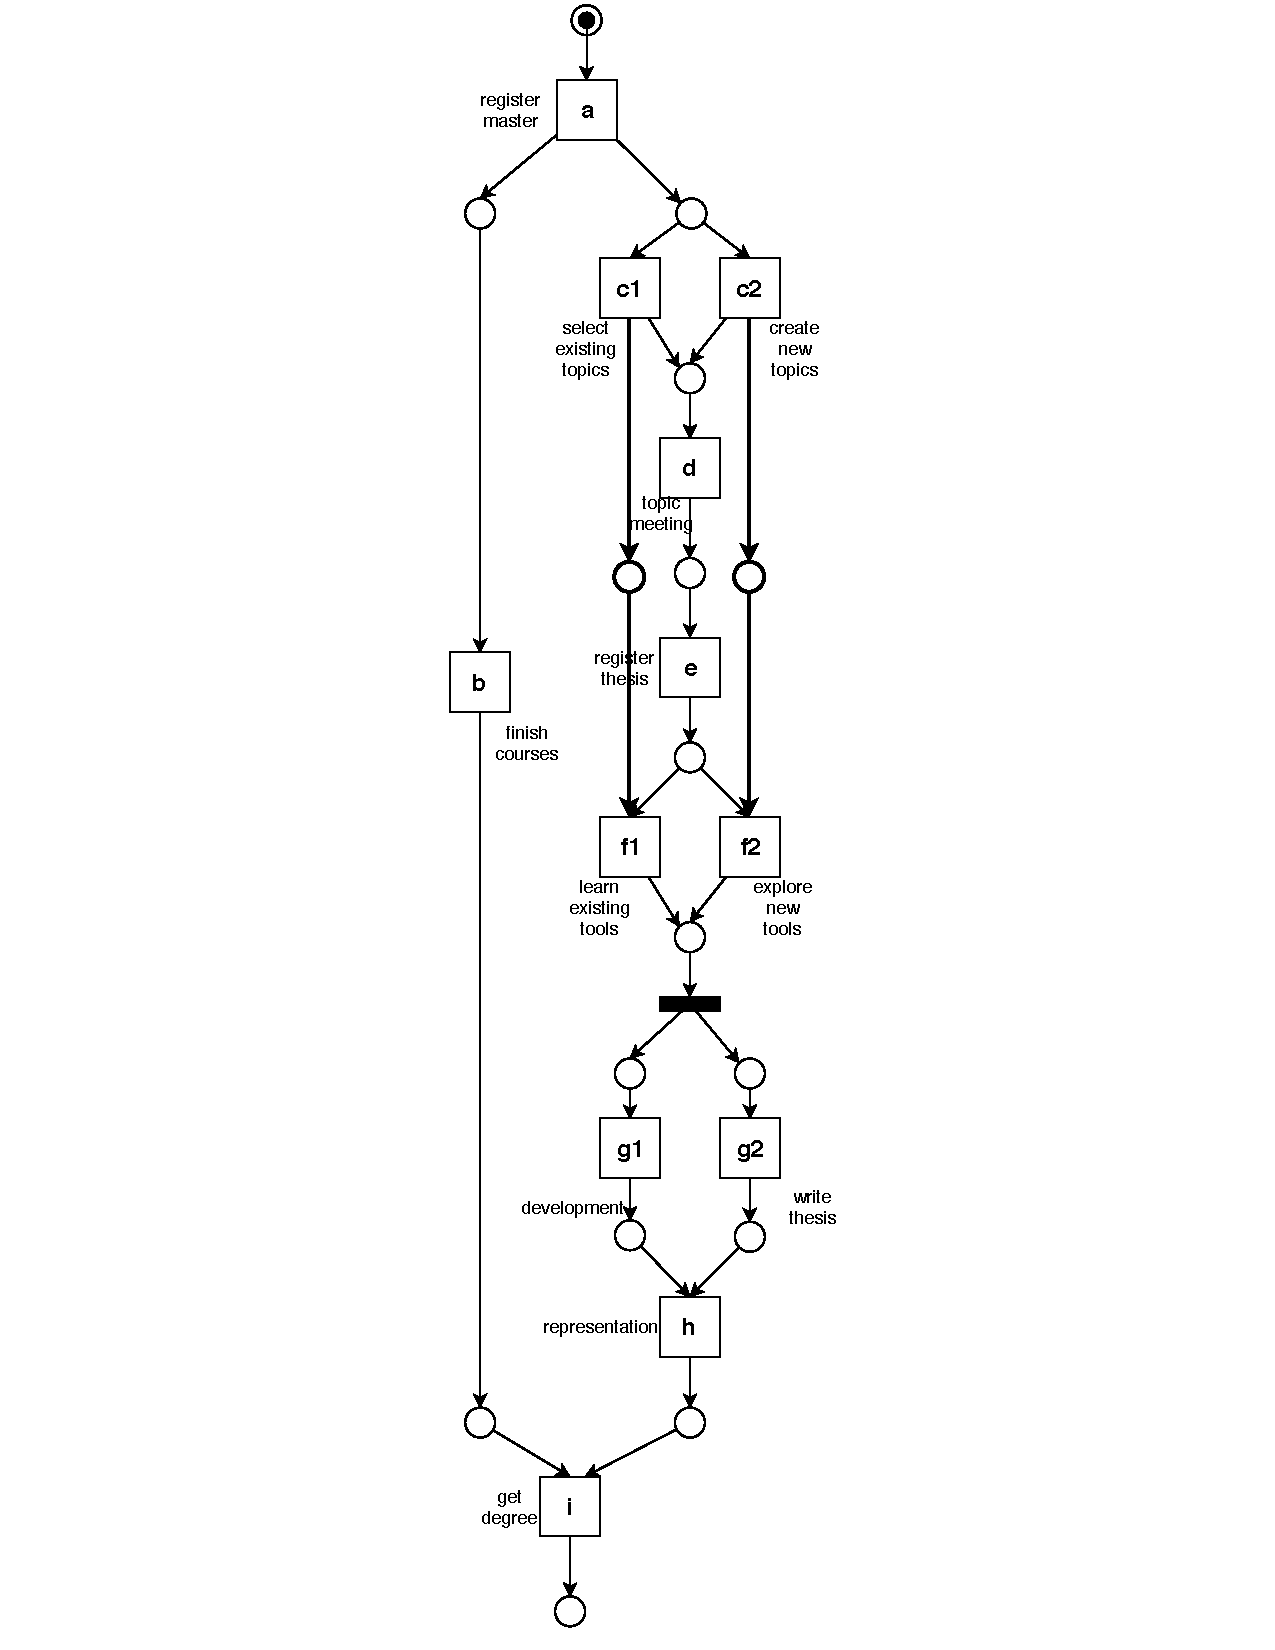
\includegraphics[clip, trim=7cm 0cm 7cm 0cm, width=0.5\linewidth, height=0.7\textheight]{figures/introduction/Master-with-lt.pdf}
		\caption{model $M_{3}$ with long-term dependency}
		\label{fig:model_d}
	\end{subfigure}
	\caption{example for situation 2 and 3}
	\label{fig:model_changes_2_3}
\end{figure}
\subsection{Situation 3: \small{Detecting Long-term Dependency}}
Another problem is that current methods are unable to detect the long-term dependency in the Petri net, which causes a lower precision. The long-term dependency describes the phenomenon that the execution of an activity decides the execution of activities that do not follow directly. Due to the long distance of this dependency, current methods cannot detect it and improve the precision by adding long-term dependency on the model. One example  on $M_0$ is used to demonstrate this problem.
 

When using time consumption on the whole study as one KPI, if the total sum goes over one threshold, the trace is negative, else as positive. Since the activity \textbf{create new topics} usually demands new knowledge rather than \textbf{checking the existing tools}. If students choose to learn existing tools, it's possibly not useful and time-wasting. In the other case, if we select existing topics with existing background, it saves time when we directly learn the existing tools. According to this performance standard, we classified those event traces into positive and negative shown above.
%here we list one example to explain the long-term dependency, but we need to make them clear, might without the loop item..It means that we need to change the whole model..
An event log $L_3$ is given in the following. 
\begin{align*}
L_3:= \{ & { <a,b,\textbf{c1},d,e,\textbf{f1},g1,g2, h,i>}^{50, pos}, \\   &{<a,b,\textbf{c2},d,e,\textbf{f2},g2,g1, h,i>}^{50, pos} ; \\
& {<a,b,\textbf{c1},d,e,\textbf{f2},g2,g1,h,i>}^{50, neg}, \\
& {<a,b,\textbf{c2},d,e,\textbf{f1},g1,g2,h,i>}^{50, neg}  \}
\end{align*}


There are no deviations of the model and event log $L_3$ according to the  algorithms in  \cite{fahland2015model} and  \cite{dees2017enhancing}. Therefore, the original model stays the same and allows for the execution of negative instances. After checking the model and log, those long-term dependencies are significant. Transition \textbf{\emph{c1}} decides \textbf{\emph{f1}} while \textbf{\emph{c2}} decides \textbf{\emph{f2}}.  After addressing long-term dependency like the model $M_3$ in Figure \ref{fig:model_d} by connecting transitions to extra places, 
negative instances are blocked and the model has higher precision.

Clearly, the use of negative information can bring significant benefits, e.g, enable a controlled generalization of a process model: the patterns to generalize should never include negative instances. This leads to the demand of improving current repair model techniques with incorporating negative instances. In the next section, the demand is analyzed and defined in a formal way.

\section{Research Scope And Questions }
After analyzing the current model repair methods, we limit our research scope as shown in Figure \ref{fig:scope}.  The inputs for our research are one existing process model M, an event log L . According to predefined KPIs, each trace in event log is classified into positive or negative. After applying repair techniques in the black box, the model should be improved to enforce the positive instances while disallowing negative instance, with condition that the generated model should be as similar to the original model as possible. 
\begin{figure}
	\centering
	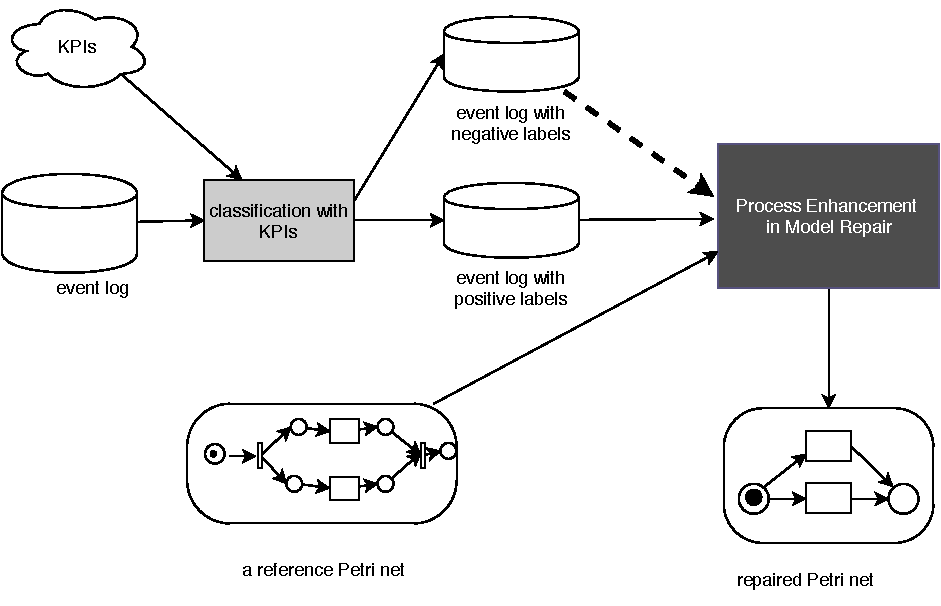
\includegraphics[width=\textwidth]{figures/introduction/P06-problem-scope.pdf}
	\caption{The resaerch problem scope}
	\label{fig:scope}
\end{figure}

In this scope, we come up with several research questions listed in the following.
\begin{enumerate}[start=1,label={\bfseries{ RQ\arabic*:}}]
	%\itemsep0em
	\item How to overcome the shortcomings of current repair techniques in situations 1-3 above?
	\item How to balance the impact of the existing model, negative and positive instances together to repair model? 
	\item How to block negative instances from the model while enforcing the positive ones?
\end{enumerate}
  
In this thesis, we propose a solution for the black box. It analyzes process performance on trace level and balances the existing model, positive traces and negative traces on directly-follows relation, to incorporate all the factors on model generation. 

\section{Outline}
This thesis aims to answer the questions presented in section 1.2 in the remaining chapters and provides a solution for the black box. 
Chapter 2 introduces the related works. Chapter 3 recalls the basic notions on process mining and list the preliminaries to solve the problem. 
Chapter 4 firstly presents an original framework to incorporate negative information into model repair. Based on this framework, a concrete algorithm are proposed. 
In Chapter 5, screenshots of the implementation tools are shown to demonstrate the usage.  Chapter 6 answers the last question RQ3, by conducting a bundle of experiments. Later, results are analyzed and discussed. 
At last, we summarize our work in Chapter 7. 
%The next section answers the questions, how to balance all factors and block negative instances, Our algorithm analyzes process performance on trace level and balances the existing model, positive traces and negative traces on directly-follows relation, in order to incorporate all the factors on model generation. Long-term dependency is further detected on the intermediate model and added to block negative instances. What's more, the impact of the existing model, positive and negative instances are parameterized by weights, to allow more flexibility of the generated model.



%\end{document}